% =====================================================================
% Representational Drift Across Versions
% Numbers from runs/qwen05b_cpu/drift.json (64-token, 32-seq anchors) with
% a replication in runs/qwen05b_agnews/drift.json (32-token, 16-seq anchors).
% TODO(GPU): replace with the 1.5B pair (runs/qwen2_to_qwen25_1.5b/drift.json)
% and add the drift-vs-naive-degradation correlation panel.
% =====================================================================
\section{Representational Drift Across Versions}
\label{sec:drift}

Before asking whether an adapter can be re-aligned, we ask whether there is
anything to align: does a same-family version bump actually move the
activation geometry of the adapted modules, and if so, where? We measure
$\mathrm{drift}_\ell=1-\mathrm{CKA}(H^{\mathrm{in},v}_\ell,H^{\mathrm{in},v+1}_\ell)$
(Eq.~\ref{eq:cka}) on the input activations of all 96 LoRA-target modules
($\{q,k,v,o\}$-projections across 24 layers) of
Qwen2-0.5B\,$\to$\,Qwen2.5-0.5B over a WikiText-2 anchor set. Because linear
CKA is invariant to orthogonal transformations of either side, a nonzero value
certifies that the two versions differ by more than a rotation.
%TODO(GPU): same figure for the 1.5B pair.

\begin{figure}[t]
\centering
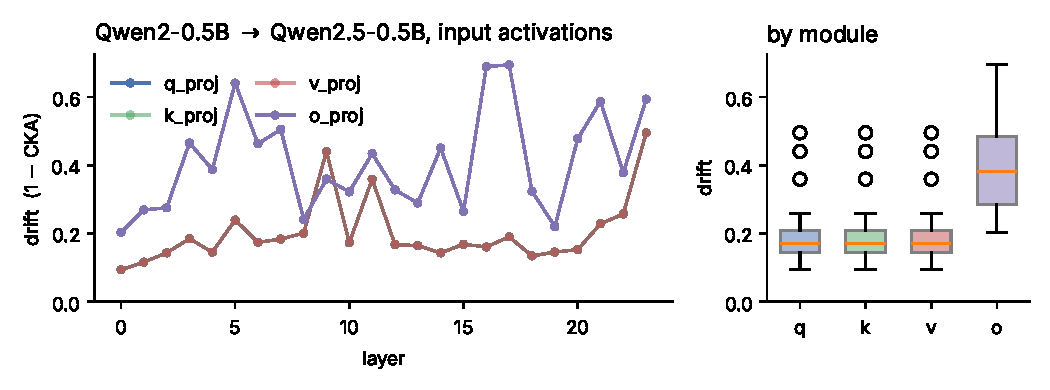
\includegraphics[width=\linewidth]{figures/drift_qwen05b.pdf}
\caption{Per-module representational drift, $1-\mathrm{CKA}$ of input
activations between Qwen2-0.5B and Qwen2.5-0.5B over unlabeled anchors.
Left: drift by layer for each projection; $q$, $k$, $v$ share an input (the
post-norm residual stream) and coincide, while $o$\_proj reads the attention
output. Right: distribution per module type. Drift is nonzero everywhere, grows
with depth, and is roughly twice as large at $o$\_proj as at the residual-stream
projections.}
\label{fig:drift}
\end{figure}

\paragraph{Drift is nonzero everywhere and grows with depth.}
Figure~\ref{fig:drift} summarizes the measurement. Mean drift over the 96
modules is $0.25$, with a minimum of $0.09$ at the layer-0 $q/k/v$ inputs and a
maximum of $0.69$ at an $o$\_proj in layer 17. No module is unchanged: even the
first layer, whose input is the token embedding after one normalization,
differs between the two versions by a non-orthogonal transformation. Averaged
over module types, drift rises from $0.12$ in layer~0 to $0.52$ in layer~23,
with a non-monotone profile in the middle of the network (local peaks at layers
5, 9, 11, 17, and 21). The replication with a smaller anchor set
(16 sequences of 32 tokens) reproduces the ordering and the depth trend with
uniformly lower magnitudes (mean $0.18$), as expected when the anchor sample is
too small to resolve the full covariance.

\paragraph{The attention-output projection drifts most.}
The input to $o$\_proj is the concatenated attention output, and it drifts about
twice as much as the residual stream read by $q$, $k$, and $v$ ($0.41$ versus
$0.20$ on average). This is consistent with the version update having changed
attention behaviour (which heads attend where, and how value vectors are
organized) more than it changed the residual-stream basis itself. For adapter
transfer it has a direct consequence: the $B$ factor of a $v$\_proj adapter and
the $A$ factor of an $o$\_proj adapter both live in exactly this most-drifted
space, so a method that corrects only the residual-stream side would miss the
largest component of the mismatch.

\paragraph{Why this matters for weight-only alignment.}
Drift as measured here is a statement about what the modules compute on real
inputs, not about their weight matrices. A method that relates two versions
through the singular subspaces of $W_\ell$ alone (\S\ref{sec:method:crosslora})
cannot observe the quantity in Figure~\ref{fig:drift}: a change in the
distribution of inputs reaching $W_\ell$, produced by every layer upstream,
leaves $W_\ell$'s SVD untouched. The experiments in \S\ref{sec:experiments}
test whether that blind spot costs accuracy.

\paragraph{Drift predicts naive-transfer failure.}
%TODO(GPU): per-module ablation -- transplant only module l naively, measure
% degradation, correlate with drift_l. Needs the 1.5B run. Keep this paragraph
% as a placeholder until runs/qwen2_to_qwen25_1.5b/drift_vs_naive.json exists.
If drift is the mechanism behind the failure of naive transfer, modules with
larger drift should account for more of the degradation when their adapter
factors are dropped onto $M_{v+1}$ unchanged. We test this by transplanting one
module's factors at a time and correlating the resulting loss increase with
$\mathrm{drift}_\ell$; results are reported with the main experiments.
